\documentclass[11pt]{article}

    \usepackage[breakable]{tcolorbox}
    \usepackage{parskip} % Stop auto-indenting (to mimic markdown behaviour)
    
    \usepackage{iftex}
    \ifPDFTeX
    	\usepackage[T1]{fontenc}
    	\usepackage{mathpazo}
    \else
    	\usepackage{fontspec}
    \fi

    % Basic figure setup, for now with no caption control since it's done
    % automatically by Pandoc (which extracts ![](path) syntax from Markdown).
    \usepackage{graphicx}
    % Maintain compatibility with old templates. Remove in nbconvert 6.0
    \let\Oldincludegraphics\includegraphics
    % Ensure that by default, figures have no caption (until we provide a
    % proper Figure object with a Caption API and a way to capture that
    % in the conversion process - todo).
    \usepackage{caption}
    \DeclareCaptionFormat{nocaption}{}
    \captionsetup{format=nocaption,aboveskip=0pt,belowskip=0pt}

    \usepackage[Export]{adjustbox} % Used to constrain images to a maximum size
    \adjustboxset{max size={0.9\linewidth}{0.9\paperheight}}
    \usepackage{float}
    \floatplacement{figure}{H} % forces figures to be placed at the correct location
    \usepackage{xcolor} % Allow colors to be defined
    \usepackage{enumerate} % Needed for markdown enumerations to work
    \usepackage{geometry} % Used to adjust the document margins
    \usepackage{amsmath} % Equations
    \usepackage{amssymb} % Equations
    \usepackage{textcomp} % defines textquotesingle
    % Hack from http://tex.stackexchange.com/a/47451/13684:
    \AtBeginDocument{%
        \def\PYZsq{\textquotesingle}% Upright quotes in Pygmentized code
    }
    \usepackage{upquote} % Upright quotes for verbatim code
    \usepackage{eurosym} % defines \euro
    \usepackage[mathletters]{ucs} % Extended unicode (utf-8) support
    \usepackage{fancyvrb} % verbatim replacement that allows latex
    \usepackage{grffile} % extends the file name processing of package graphics 
                         % to support a larger range
    \makeatletter % fix for grffile with XeLaTeX
    \def\Gread@@xetex#1{%
      \IfFileExists{"\Gin@base".bb}%
      {\Gread@eps{\Gin@base.bb}}%
      {\Gread@@xetex@aux#1}%
    }
    \makeatother

    % The hyperref package gives us a pdf with properly built
    % internal navigation ('pdf bookmarks' for the table of contents,
    % internal cross-reference links, web links for URLs, etc.)
    \usepackage{hyperref}
    % The default LaTeX title has an obnoxious amount of whitespace. By default,
    % titling removes some of it. It also provides customization options.
    \usepackage{titling}
    \usepackage{longtable} % longtable support required by pandoc >1.10
    \usepackage{booktabs}  % table support for pandoc > 1.12.2
    \usepackage[inline]{enumitem} % IRkernel/repr support (it uses the enumerate* environment)
    \usepackage[normalem]{ulem} % ulem is needed to support strikethroughs (\sout)
                                % normalem makes italics be italics, not underlines
    \usepackage{mathrsfs}
    

    
    % Colors for the hyperref package
    \definecolor{urlcolor}{rgb}{0,.145,.698}
    \definecolor{linkcolor}{rgb}{.71,0.21,0.01}
    \definecolor{citecolor}{rgb}{.12,.54,.11}

    % ANSI colors
    \definecolor{ansi-black}{HTML}{3E424D}
    \definecolor{ansi-black-intense}{HTML}{282C36}
    \definecolor{ansi-red}{HTML}{E75C58}
    \definecolor{ansi-red-intense}{HTML}{B22B31}
    \definecolor{ansi-green}{HTML}{00A250}
    \definecolor{ansi-green-intense}{HTML}{007427}
    \definecolor{ansi-yellow}{HTML}{DDB62B}
    \definecolor{ansi-yellow-intense}{HTML}{B27D12}
    \definecolor{ansi-blue}{HTML}{208FFB}
    \definecolor{ansi-blue-intense}{HTML}{0065CA}
    \definecolor{ansi-magenta}{HTML}{D160C4}
    \definecolor{ansi-magenta-intense}{HTML}{A03196}
    \definecolor{ansi-cyan}{HTML}{60C6C8}
    \definecolor{ansi-cyan-intense}{HTML}{258F8F}
    \definecolor{ansi-white}{HTML}{C5C1B4}
    \definecolor{ansi-white-intense}{HTML}{A1A6B2}
    \definecolor{ansi-default-inverse-fg}{HTML}{FFFFFF}
    \definecolor{ansi-default-inverse-bg}{HTML}{000000}

    % commands and environments needed by pandoc snippets
    % extracted from the output of `pandoc -s`
    \providecommand{\tightlist}{%
      \setlength{\itemsep}{0pt}\setlength{\parskip}{0pt}}
    \DefineVerbatimEnvironment{Highlighting}{Verbatim}{commandchars=\\\{\}}
    % Add ',fontsize=\small' for more characters per line
    \newenvironment{Shaded}{}{}
    \newcommand{\KeywordTok}[1]{\textcolor[rgb]{0.00,0.44,0.13}{\textbf{{#1}}}}
    \newcommand{\DataTypeTok}[1]{\textcolor[rgb]{0.56,0.13,0.00}{{#1}}}
    \newcommand{\DecValTok}[1]{\textcolor[rgb]{0.25,0.63,0.44}{{#1}}}
    \newcommand{\BaseNTok}[1]{\textcolor[rgb]{0.25,0.63,0.44}{{#1}}}
    \newcommand{\FloatTok}[1]{\textcolor[rgb]{0.25,0.63,0.44}{{#1}}}
    \newcommand{\CharTok}[1]{\textcolor[rgb]{0.25,0.44,0.63}{{#1}}}
    \newcommand{\StringTok}[1]{\textcolor[rgb]{0.25,0.44,0.63}{{#1}}}
    \newcommand{\CommentTok}[1]{\textcolor[rgb]{0.38,0.63,0.69}{\textit{{#1}}}}
    \newcommand{\OtherTok}[1]{\textcolor[rgb]{0.00,0.44,0.13}{{#1}}}
    \newcommand{\AlertTok}[1]{\textcolor[rgb]{1.00,0.00,0.00}{\textbf{{#1}}}}
    \newcommand{\FunctionTok}[1]{\textcolor[rgb]{0.02,0.16,0.49}{{#1}}}
    \newcommand{\RegionMarkerTok}[1]{{#1}}
    \newcommand{\ErrorTok}[1]{\textcolor[rgb]{1.00,0.00,0.00}{\textbf{{#1}}}}
    \newcommand{\NormalTok}[1]{{#1}}
    
    % Additional commands for more recent versions of Pandoc
    \newcommand{\ConstantTok}[1]{\textcolor[rgb]{0.53,0.00,0.00}{{#1}}}
    \newcommand{\SpecialCharTok}[1]{\textcolor[rgb]{0.25,0.44,0.63}{{#1}}}
    \newcommand{\VerbatimStringTok}[1]{\textcolor[rgb]{0.25,0.44,0.63}{{#1}}}
    \newcommand{\SpecialStringTok}[1]{\textcolor[rgb]{0.73,0.40,0.53}{{#1}}}
    \newcommand{\ImportTok}[1]{{#1}}
    \newcommand{\DocumentationTok}[1]{\textcolor[rgb]{0.73,0.13,0.13}{\textit{{#1}}}}
    \newcommand{\AnnotationTok}[1]{\textcolor[rgb]{0.38,0.63,0.69}{\textbf{\textit{{#1}}}}}
    \newcommand{\CommentVarTok}[1]{\textcolor[rgb]{0.38,0.63,0.69}{\textbf{\textit{{#1}}}}}
    \newcommand{\VariableTok}[1]{\textcolor[rgb]{0.10,0.09,0.49}{{#1}}}
    \newcommand{\ControlFlowTok}[1]{\textcolor[rgb]{0.00,0.44,0.13}{\textbf{{#1}}}}
    \newcommand{\OperatorTok}[1]{\textcolor[rgb]{0.40,0.40,0.40}{{#1}}}
    \newcommand{\BuiltInTok}[1]{{#1}}
    \newcommand{\ExtensionTok}[1]{{#1}}
    \newcommand{\PreprocessorTok}[1]{\textcolor[rgb]{0.74,0.48,0.00}{{#1}}}
    \newcommand{\AttributeTok}[1]{\textcolor[rgb]{0.49,0.56,0.16}{{#1}}}
    \newcommand{\InformationTok}[1]{\textcolor[rgb]{0.38,0.63,0.69}{\textbf{\textit{{#1}}}}}
    \newcommand{\WarningTok}[1]{\textcolor[rgb]{0.38,0.63,0.69}{\textbf{\textit{{#1}}}}}
    
    
    % Define a nice break command that doesn't care if a line doesn't already
    % exist.
    \def\br{\hspace*{\fill} \\* }
    % Math Jax compatibility definitions
    \def\gt{>}
    \def\lt{<}
    \let\Oldtex\TeX
    \let\Oldlatex\LaTeX
    \renewcommand{\TeX}{\textrm{\Oldtex}}
    \renewcommand{\LaTeX}{\textrm{\Oldlatex}}
    % Document parameters
    % Document title
    \title{Chapter7\_Stability}
    
    
    
    
    
% Pygments definitions
\makeatletter
\def\PY@reset{\let\PY@it=\relax \let\PY@bf=\relax%
    \let\PY@ul=\relax \let\PY@tc=\relax%
    \let\PY@bc=\relax \let\PY@ff=\relax}
\def\PY@tok#1{\csname PY@tok@#1\endcsname}
\def\PY@toks#1+{\ifx\relax#1\empty\else%
    \PY@tok{#1}\expandafter\PY@toks\fi}
\def\PY@do#1{\PY@bc{\PY@tc{\PY@ul{%
    \PY@it{\PY@bf{\PY@ff{#1}}}}}}}
\def\PY#1#2{\PY@reset\PY@toks#1+\relax+\PY@do{#2}}

\expandafter\def\csname PY@tok@s\endcsname{\def\PY@tc##1{\textcolor[rgb]{0.73,0.13,0.13}{##1}}}
\expandafter\def\csname PY@tok@ni\endcsname{\let\PY@bf=\textbf\def\PY@tc##1{\textcolor[rgb]{0.60,0.60,0.60}{##1}}}
\expandafter\def\csname PY@tok@vg\endcsname{\def\PY@tc##1{\textcolor[rgb]{0.10,0.09,0.49}{##1}}}
\expandafter\def\csname PY@tok@s1\endcsname{\def\PY@tc##1{\textcolor[rgb]{0.73,0.13,0.13}{##1}}}
\expandafter\def\csname PY@tok@ch\endcsname{\let\PY@it=\textit\def\PY@tc##1{\textcolor[rgb]{0.25,0.50,0.50}{##1}}}
\expandafter\def\csname PY@tok@err\endcsname{\def\PY@bc##1{\setlength{\fboxsep}{0pt}\fcolorbox[rgb]{1.00,0.00,0.00}{1,1,1}{\strut ##1}}}
\expandafter\def\csname PY@tok@vc\endcsname{\def\PY@tc##1{\textcolor[rgb]{0.10,0.09,0.49}{##1}}}
\expandafter\def\csname PY@tok@nv\endcsname{\def\PY@tc##1{\textcolor[rgb]{0.10,0.09,0.49}{##1}}}
\expandafter\def\csname PY@tok@nd\endcsname{\def\PY@tc##1{\textcolor[rgb]{0.67,0.13,1.00}{##1}}}
\expandafter\def\csname PY@tok@nn\endcsname{\let\PY@bf=\textbf\def\PY@tc##1{\textcolor[rgb]{0.00,0.00,1.00}{##1}}}
\expandafter\def\csname PY@tok@mb\endcsname{\def\PY@tc##1{\textcolor[rgb]{0.40,0.40,0.40}{##1}}}
\expandafter\def\csname PY@tok@si\endcsname{\let\PY@bf=\textbf\def\PY@tc##1{\textcolor[rgb]{0.73,0.40,0.53}{##1}}}
\expandafter\def\csname PY@tok@c\endcsname{\let\PY@it=\textit\def\PY@tc##1{\textcolor[rgb]{0.25,0.50,0.50}{##1}}}
\expandafter\def\csname PY@tok@gd\endcsname{\def\PY@tc##1{\textcolor[rgb]{0.63,0.00,0.00}{##1}}}
\expandafter\def\csname PY@tok@nf\endcsname{\def\PY@tc##1{\textcolor[rgb]{0.00,0.00,1.00}{##1}}}
\expandafter\def\csname PY@tok@kt\endcsname{\def\PY@tc##1{\textcolor[rgb]{0.69,0.00,0.25}{##1}}}
\expandafter\def\csname PY@tok@nc\endcsname{\let\PY@bf=\textbf\def\PY@tc##1{\textcolor[rgb]{0.00,0.00,1.00}{##1}}}
\expandafter\def\csname PY@tok@m\endcsname{\def\PY@tc##1{\textcolor[rgb]{0.40,0.40,0.40}{##1}}}
\expandafter\def\csname PY@tok@sx\endcsname{\def\PY@tc##1{\textcolor[rgb]{0.00,0.50,0.00}{##1}}}
\expandafter\def\csname PY@tok@mi\endcsname{\def\PY@tc##1{\textcolor[rgb]{0.40,0.40,0.40}{##1}}}
\expandafter\def\csname PY@tok@vi\endcsname{\def\PY@tc##1{\textcolor[rgb]{0.10,0.09,0.49}{##1}}}
\expandafter\def\csname PY@tok@ow\endcsname{\let\PY@bf=\textbf\def\PY@tc##1{\textcolor[rgb]{0.67,0.13,1.00}{##1}}}
\expandafter\def\csname PY@tok@go\endcsname{\def\PY@tc##1{\textcolor[rgb]{0.53,0.53,0.53}{##1}}}
\expandafter\def\csname PY@tok@gh\endcsname{\let\PY@bf=\textbf\def\PY@tc##1{\textcolor[rgb]{0.00,0.00,0.50}{##1}}}
\expandafter\def\csname PY@tok@nb\endcsname{\def\PY@tc##1{\textcolor[rgb]{0.00,0.50,0.00}{##1}}}
\expandafter\def\csname PY@tok@nl\endcsname{\def\PY@tc##1{\textcolor[rgb]{0.63,0.63,0.00}{##1}}}
\expandafter\def\csname PY@tok@sc\endcsname{\def\PY@tc##1{\textcolor[rgb]{0.73,0.13,0.13}{##1}}}
\expandafter\def\csname PY@tok@se\endcsname{\let\PY@bf=\textbf\def\PY@tc##1{\textcolor[rgb]{0.73,0.40,0.13}{##1}}}
\expandafter\def\csname PY@tok@gi\endcsname{\def\PY@tc##1{\textcolor[rgb]{0.00,0.63,0.00}{##1}}}
\expandafter\def\csname PY@tok@s2\endcsname{\def\PY@tc##1{\textcolor[rgb]{0.73,0.13,0.13}{##1}}}
\expandafter\def\csname PY@tok@il\endcsname{\def\PY@tc##1{\textcolor[rgb]{0.40,0.40,0.40}{##1}}}
\expandafter\def\csname PY@tok@o\endcsname{\def\PY@tc##1{\textcolor[rgb]{0.40,0.40,0.40}{##1}}}
\expandafter\def\csname PY@tok@cp\endcsname{\def\PY@tc##1{\textcolor[rgb]{0.74,0.48,0.00}{##1}}}
\expandafter\def\csname PY@tok@sd\endcsname{\let\PY@it=\textit\def\PY@tc##1{\textcolor[rgb]{0.73,0.13,0.13}{##1}}}
\expandafter\def\csname PY@tok@sr\endcsname{\def\PY@tc##1{\textcolor[rgb]{0.73,0.40,0.53}{##1}}}
\expandafter\def\csname PY@tok@gt\endcsname{\def\PY@tc##1{\textcolor[rgb]{0.00,0.27,0.87}{##1}}}
\expandafter\def\csname PY@tok@cpf\endcsname{\let\PY@it=\textit\def\PY@tc##1{\textcolor[rgb]{0.25,0.50,0.50}{##1}}}
\expandafter\def\csname PY@tok@nt\endcsname{\let\PY@bf=\textbf\def\PY@tc##1{\textcolor[rgb]{0.00,0.50,0.00}{##1}}}
\expandafter\def\csname PY@tok@cm\endcsname{\let\PY@it=\textit\def\PY@tc##1{\textcolor[rgb]{0.25,0.50,0.50}{##1}}}
\expandafter\def\csname PY@tok@w\endcsname{\def\PY@tc##1{\textcolor[rgb]{0.73,0.73,0.73}{##1}}}
\expandafter\def\csname PY@tok@mh\endcsname{\def\PY@tc##1{\textcolor[rgb]{0.40,0.40,0.40}{##1}}}
\expandafter\def\csname PY@tok@na\endcsname{\def\PY@tc##1{\textcolor[rgb]{0.49,0.56,0.16}{##1}}}
\expandafter\def\csname PY@tok@kc\endcsname{\let\PY@bf=\textbf\def\PY@tc##1{\textcolor[rgb]{0.00,0.50,0.00}{##1}}}
\expandafter\def\csname PY@tok@kn\endcsname{\let\PY@bf=\textbf\def\PY@tc##1{\textcolor[rgb]{0.00,0.50,0.00}{##1}}}
\expandafter\def\csname PY@tok@fm\endcsname{\def\PY@tc##1{\textcolor[rgb]{0.00,0.00,1.00}{##1}}}
\expandafter\def\csname PY@tok@sh\endcsname{\def\PY@tc##1{\textcolor[rgb]{0.73,0.13,0.13}{##1}}}
\expandafter\def\csname PY@tok@gs\endcsname{\let\PY@bf=\textbf}
\expandafter\def\csname PY@tok@sb\endcsname{\def\PY@tc##1{\textcolor[rgb]{0.73,0.13,0.13}{##1}}}
\expandafter\def\csname PY@tok@ne\endcsname{\let\PY@bf=\textbf\def\PY@tc##1{\textcolor[rgb]{0.82,0.25,0.23}{##1}}}
\expandafter\def\csname PY@tok@cs\endcsname{\let\PY@it=\textit\def\PY@tc##1{\textcolor[rgb]{0.25,0.50,0.50}{##1}}}
\expandafter\def\csname PY@tok@sa\endcsname{\def\PY@tc##1{\textcolor[rgb]{0.73,0.13,0.13}{##1}}}
\expandafter\def\csname PY@tok@kp\endcsname{\def\PY@tc##1{\textcolor[rgb]{0.00,0.50,0.00}{##1}}}
\expandafter\def\csname PY@tok@no\endcsname{\def\PY@tc##1{\textcolor[rgb]{0.53,0.00,0.00}{##1}}}
\expandafter\def\csname PY@tok@vm\endcsname{\def\PY@tc##1{\textcolor[rgb]{0.10,0.09,0.49}{##1}}}
\expandafter\def\csname PY@tok@gu\endcsname{\let\PY@bf=\textbf\def\PY@tc##1{\textcolor[rgb]{0.50,0.00,0.50}{##1}}}
\expandafter\def\csname PY@tok@gp\endcsname{\let\PY@bf=\textbf\def\PY@tc##1{\textcolor[rgb]{0.00,0.00,0.50}{##1}}}
\expandafter\def\csname PY@tok@mf\endcsname{\def\PY@tc##1{\textcolor[rgb]{0.40,0.40,0.40}{##1}}}
\expandafter\def\csname PY@tok@dl\endcsname{\def\PY@tc##1{\textcolor[rgb]{0.73,0.13,0.13}{##1}}}
\expandafter\def\csname PY@tok@c1\endcsname{\let\PY@it=\textit\def\PY@tc##1{\textcolor[rgb]{0.25,0.50,0.50}{##1}}}
\expandafter\def\csname PY@tok@gr\endcsname{\def\PY@tc##1{\textcolor[rgb]{1.00,0.00,0.00}{##1}}}
\expandafter\def\csname PY@tok@ss\endcsname{\def\PY@tc##1{\textcolor[rgb]{0.10,0.09,0.49}{##1}}}
\expandafter\def\csname PY@tok@ge\endcsname{\let\PY@it=\textit}
\expandafter\def\csname PY@tok@kr\endcsname{\let\PY@bf=\textbf\def\PY@tc##1{\textcolor[rgb]{0.00,0.50,0.00}{##1}}}
\expandafter\def\csname PY@tok@bp\endcsname{\def\PY@tc##1{\textcolor[rgb]{0.00,0.50,0.00}{##1}}}
\expandafter\def\csname PY@tok@mo\endcsname{\def\PY@tc##1{\textcolor[rgb]{0.40,0.40,0.40}{##1}}}
\expandafter\def\csname PY@tok@k\endcsname{\let\PY@bf=\textbf\def\PY@tc##1{\textcolor[rgb]{0.00,0.50,0.00}{##1}}}
\expandafter\def\csname PY@tok@kd\endcsname{\let\PY@bf=\textbf\def\PY@tc##1{\textcolor[rgb]{0.00,0.50,0.00}{##1}}}

\def\PYZbs{\char`\\}
\def\PYZus{\char`\_}
\def\PYZob{\char`\{}
\def\PYZcb{\char`\}}
\def\PYZca{\char`\^}
\def\PYZam{\char`\&}
\def\PYZlt{\char`\<}
\def\PYZgt{\char`\>}
\def\PYZsh{\char`\#}
\def\PYZpc{\char`\%}
\def\PYZdl{\char`\$}
\def\PYZhy{\char`\-}
\def\PYZsq{\char`\'}
\def\PYZdq{\char`\"}
\def\PYZti{\char`\~}
% for compatibility with earlier versions
\def\PYZat{@}
\def\PYZlb{[}
\def\PYZrb{]}
\makeatother


    % For linebreaks inside Verbatim environment from package fancyvrb. 
    \makeatletter
        \newbox\Wrappedcontinuationbox 
        \newbox\Wrappedvisiblespacebox 
        \newcommand*\Wrappedvisiblespace {\textcolor{red}{\textvisiblespace}} 
        \newcommand*\Wrappedcontinuationsymbol {\textcolor{red}{\llap{\tiny$\m@th\hookrightarrow$}}} 
        \newcommand*\Wrappedcontinuationindent {3ex } 
        \newcommand*\Wrappedafterbreak {\kern\Wrappedcontinuationindent\copy\Wrappedcontinuationbox} 
        % Take advantage of the already applied Pygments mark-up to insert 
        % potential linebreaks for TeX processing. 
        %        {, <, #, %, $, ' and ": go to next line. 
        %        _, }, ^, &, >, - and ~: stay at end of broken line. 
        % Use of \textquotesingle for straight quote. 
        \newcommand*\Wrappedbreaksatspecials {% 
            \def\PYGZus{\discretionary{\char`\_}{\Wrappedafterbreak}{\char`\_}}% 
            \def\PYGZob{\discretionary{}{\Wrappedafterbreak\char`\{}{\char`\{}}% 
            \def\PYGZcb{\discretionary{\char`\}}{\Wrappedafterbreak}{\char`\}}}% 
            \def\PYGZca{\discretionary{\char`\^}{\Wrappedafterbreak}{\char`\^}}% 
            \def\PYGZam{\discretionary{\char`\&}{\Wrappedafterbreak}{\char`\&}}% 
            \def\PYGZlt{\discretionary{}{\Wrappedafterbreak\char`\<}{\char`\<}}% 
            \def\PYGZgt{\discretionary{\char`\>}{\Wrappedafterbreak}{\char`\>}}% 
            \def\PYGZsh{\discretionary{}{\Wrappedafterbreak\char`\#}{\char`\#}}% 
            \def\PYGZpc{\discretionary{}{\Wrappedafterbreak\char`\%}{\char`\%}}% 
            \def\PYGZdl{\discretionary{}{\Wrappedafterbreak\char`\$}{\char`\$}}% 
            \def\PYGZhy{\discretionary{\char`\-}{\Wrappedafterbreak}{\char`\-}}% 
            \def\PYGZsq{\discretionary{}{\Wrappedafterbreak\textquotesingle}{\textquotesingle}}% 
            \def\PYGZdq{\discretionary{}{\Wrappedafterbreak\char`\"}{\char`\"}}% 
            \def\PYGZti{\discretionary{\char`\~}{\Wrappedafterbreak}{\char`\~}}% 
        } 
        % Some characters . , ; ? ! / are not pygmentized. 
        % This macro makes them "active" and they will insert potential linebreaks 
        \newcommand*\Wrappedbreaksatpunct {% 
            \lccode`\~`\.\lowercase{\def~}{\discretionary{\hbox{\char`\.}}{\Wrappedafterbreak}{\hbox{\char`\.}}}% 
            \lccode`\~`\,\lowercase{\def~}{\discretionary{\hbox{\char`\,}}{\Wrappedafterbreak}{\hbox{\char`\,}}}% 
            \lccode`\~`\;\lowercase{\def~}{\discretionary{\hbox{\char`\;}}{\Wrappedafterbreak}{\hbox{\char`\;}}}% 
            \lccode`\~`\:\lowercase{\def~}{\discretionary{\hbox{\char`\:}}{\Wrappedafterbreak}{\hbox{\char`\:}}}% 
            \lccode`\~`\?\lowercase{\def~}{\discretionary{\hbox{\char`\?}}{\Wrappedafterbreak}{\hbox{\char`\?}}}% 
            \lccode`\~`\!\lowercase{\def~}{\discretionary{\hbox{\char`\!}}{\Wrappedafterbreak}{\hbox{\char`\!}}}% 
            \lccode`\~`\/\lowercase{\def~}{\discretionary{\hbox{\char`\/}}{\Wrappedafterbreak}{\hbox{\char`\/}}}% 
            \catcode`\.\active
            \catcode`\,\active 
            \catcode`\;\active
            \catcode`\:\active
            \catcode`\?\active
            \catcode`\!\active
            \catcode`\/\active 
            \lccode`\~`\~ 	
        }
    \makeatother

    \let\OriginalVerbatim=\Verbatim
    \makeatletter
    \renewcommand{\Verbatim}[1][1]{%
        %\parskip\z@skip
        \sbox\Wrappedcontinuationbox {\Wrappedcontinuationsymbol}%
        \sbox\Wrappedvisiblespacebox {\FV@SetupFont\Wrappedvisiblespace}%
        \def\FancyVerbFormatLine ##1{\hsize\linewidth
            \vtop{\raggedright\hyphenpenalty\z@\exhyphenpenalty\z@
                \doublehyphendemerits\z@\finalhyphendemerits\z@
                \strut ##1\strut}%
        }%
        % If the linebreak is at a space, the latter will be displayed as visible
        % space at end of first line, and a continuation symbol starts next line.
        % Stretch/shrink are however usually zero for typewriter font.
        \def\FV@Space {%
            \nobreak\hskip\z@ plus\fontdimen3\font minus\fontdimen4\font
            \discretionary{\copy\Wrappedvisiblespacebox}{\Wrappedafterbreak}
            {\kern\fontdimen2\font}%
        }%
        
        % Allow breaks at special characters using \PYG... macros.
        \Wrappedbreaksatspecials
        % Breaks at punctuation characters . , ; ? ! and / need catcode=\active 	
        \OriginalVerbatim[#1,codes*=\Wrappedbreaksatpunct]%
    }
    \makeatother

    % Exact colors from NB
    \definecolor{incolor}{HTML}{303F9F}
    \definecolor{outcolor}{HTML}{D84315}
    \definecolor{cellborder}{HTML}{CFCFCF}
    \definecolor{cellbackground}{HTML}{F7F7F7}
    
    % prompt
    \makeatletter
    \newcommand{\boxspacing}{\kern\kvtcb@left@rule\kern\kvtcb@boxsep}
    \makeatother
    \newcommand{\prompt}[4]{
        \ttfamily\llap{{\color{#2}[#3]:\hspace{3pt}#4}}\vspace{-\baselineskip}
    }
    

    
    % Prevent overflowing lines due to hard-to-break entities
    \sloppy 
    % Setup hyperref package
    \hypersetup{
      breaklinks=true,  % so long urls are correctly broken across lines
      colorlinks=true,
      urlcolor=urlcolor,
      linkcolor=linkcolor,
      citecolor=citecolor,
      }
    % Slightly bigger margins than the latex defaults
    
    \geometry{verbose,tmargin=1in,bmargin=1in,lmargin=1in,rmargin=1in}
    
    

\begin{document}
    
    \maketitle
    
    

    
    \section{7. Stabilité}\label{stabilituxe9}

    \subsection{7.1 Introduction}\label{introduction}

    La stabilité étant essentielle à tout système en boucle fermée, il est
utile de définir des critères permettant d'établir si le système est
stable ou non.

    Le cercle unité semble jouer un rôle important pour la stabilité des
systèmes échantillonnés. Par exemple:

\begin{itemize}
\tightlist
\item
  l'étude de l'importance des pôles du chapitre 4 a montré que seuls les
  pôles à l'intérieur du cercle unité génèrent un signal amorti
\item
  l'étude de la transformation des pôles par échantillonnage a montré
  que le demi-plan gauche dans le domaine de Laplace devient l'intérieur
  du cercle unité
\end{itemize}

    \subsection{7.2 Stabilité BIBO}\label{stabilituxe9-bibo}

    \paragraph{Définition}\label{duxe9finition}

Un système discret au repos, linéaire, causal et stationnaire est BIBO
stable quand toute entrée bornée fournit une sortie bornée.

    \paragraph{Théorème}\label{thuxe9oruxe8me}

Un système discret au repos, linéaire, causal et stationnaire décrit par
une fonction de transfert rationnelle propre G(z) est BIBO stable si et
seulement si tous ses pôles sont à l'intérieur du cercle unité.

    \subsection{~7.3 Critères algébriques}\label{crituxe8res-alguxe9briques}

    \subsubsection{Critère de
Routh-Hurwitz}\label{crituxe8re-de-routh-hurwitz}

    Le critère de Routh-Hurwitz permet de vérifier que les zéros d'un
polynôme se trouvent bien dans le demi-plan complexe gauche. Afin de
pouvoir l'utiliser, il faut donc transformer le plan \(z\) vers le plan
\(s\). Pour cela, la transformation bilinéaire, ou de Möbius est
adoptée:

\[ w = \frac{z-1}{z+1} \]

dont l'inverse est:

\[ z = \frac{1+w}{1-w} \]

    Il suffit alors de vérifier que le polynôme obtenu possède bien des
pôles dans le demi-plan gauche, en appliquant le critère de
Routh-Hurwitz.

    \paragraph{Exemple 1}\label{exemple-1}

Soit le système en BO décrit par la fonction de transfert:

\[ G(z) = \frac{10^{-3}(1.23z+1.21)}{z^2-1.95z+0.95} \]

    On ajoute un régulateur de gain \(K_p\). La boucle fermée devient:

\[ \frac{Y(z)}{Y_c(z)} = \frac{10^{-3}K_p(1.23z+1.21)}{z^2+(1.23\cdot 10^{-3}K_p-1.95)z+0.95+1.21\cdot 10^{-3}K_p} \]

    Le dénominateur (polynôme caractéristique) à analyser est donc:

\[ A(z) = z^2+(1.23\cdot 10^{-3}K_p-1.95)z+0.95+1.21\cdot 10^{-3}K_p \]

    En appliquant la transformation bilinéaire, on obtient le polynôme
suivant:

\begin{align}
  A'(w) &= A\left(\frac{1+w}{1-w}\right) \\
  &= \frac{(3.9-0.02\cdot 10^{-3}K_p)w^2+(0.1-2.42\cdot 10^{-3}K_p)w+2.44\cdot 10^{-3}K_p}{w^2-2w+1}
\end{align}

    Le tableau de Routh appliqué au numérateur de \(A'(w)\) donne:

\begin{longtable}[]{@{}lll@{}}
\toprule
\( 3.9-0.02\cdot 10^{-3}K_p \) & \( 2.44\cdot 10^{-3}K_p \) &
\( 0 \)\tabularnewline
\( 0.1-2.42\cdot 10^{-3}K_p \) & \( 0 \) & \( 0 \)\tabularnewline
\( 2.44\cdot 10^{-3}K_p \) & ~\( 0 \) & \( 0 \)\tabularnewline
\( 0 \) & \( 0 \) & \( 0 \)\tabularnewline
\bottomrule
\end{longtable}

    Il faut donc que ces inégalités soient respectées:

\begin{align}
  3.9-0.02\cdot 10^{-3}K_p > 0 \\
  0.1-2.42\cdot 10^{-3}K_p > 0 \\
  2.44\cdot 10^{-3}K_p > 0
\end{align}

    Par conséquent, la stabilité en BF est garantie pour:

\[ 0 < K_p < 41.3 \] ***

    \subsubsection{Critère de Jury}\label{crituxe8re-de-jury}

    Le critère de Routh-Hurwitz étant mathématiquement lourd à utiliser en
discret à cause de la transformation bilinéaire, un autre critère existe
afin de déterminer directement si les racines d'un polynôme se trouvent
dans le cercle unité.

    Soit le polynôme à coefficients réels de degré \(n\):

\[ A(z) = a_0 z^n + a_1 z^{n-1} + \dots + a_{n-1} z + a_n \]

    Le tableau suivant est d'abord construit:

\begin{longtable}[]{@{}llllll@{}}
\toprule
\begin{minipage}[t]{0.05\columnwidth}\raggedright\strut
\[ \mathbf{a_0} \]\strut
\end{minipage} & \begin{minipage}[t]{0.05\columnwidth}\raggedright\strut
\[ a_1 \]\strut
\end{minipage} & \begin{minipage}[t]{0.05\columnwidth}\raggedright\strut
\[ \dots \]\strut
\end{minipage} & \begin{minipage}[t]{0.05\columnwidth}\raggedright\strut
\[ a_{n-1} \]\strut
\end{minipage} & \begin{minipage}[t]{0.05\columnwidth}\raggedright\strut
\[ a_n \]\strut
\end{minipage} & \begin{minipage}[t]{0.05\columnwidth}\raggedright\strut
\strut
\end{minipage}\tabularnewline
\begin{minipage}[t]{0.05\columnwidth}\raggedright\strut
\[ a_n \]\strut
\end{minipage} & \begin{minipage}[t]{0.05\columnwidth}\raggedright\strut
\[ a_{n-1} \]\strut
\end{minipage} & \begin{minipage}[t]{0.05\columnwidth}\raggedright\strut
\[ \dots \]\strut
\end{minipage} & \begin{minipage}[t]{0.05\columnwidth}\raggedright\strut
\[ a_1 \]\strut
\end{minipage} & \begin{minipage}[t]{0.05\columnwidth}\raggedright\strut
\[ a_0 \]\strut
\end{minipage} & \begin{minipage}[t]{0.05\columnwidth}\raggedright\strut
\[ \alpha_n = \frac{a_n}{a_0} \]\strut
\end{minipage}\tabularnewline
\begin{minipage}[t]{0.05\columnwidth}\raggedright\strut
\[ \mathbf{a_0^{(n-1)}} \]\strut
\end{minipage} & \begin{minipage}[t]{0.05\columnwidth}\raggedright\strut
\[ a_1^{(n-1)} \]\strut
\end{minipage} & \begin{minipage}[t]{0.05\columnwidth}\raggedright\strut
\[ \dots \]\strut
\end{minipage} & \begin{minipage}[t]{0.05\columnwidth}\raggedright\strut
\[ a_{n-1}^{(n-1)} \]\strut
\end{minipage} & \begin{minipage}[t]{0.05\columnwidth}\raggedright\strut
\strut
\end{minipage} & \begin{minipage}[t]{0.05\columnwidth}\raggedright\strut
\strut
\end{minipage}\tabularnewline
\begin{minipage}[t]{0.05\columnwidth}\raggedright\strut
\[ a_{n-1}^{(n-1)} \]\strut
\end{minipage} & \begin{minipage}[t]{0.05\columnwidth}\raggedright\strut
\[ a_{n-2}^{(n-1)} \]\strut
\end{minipage} & \begin{minipage}[t]{0.05\columnwidth}\raggedright\strut
\[ \dots \]\strut
\end{minipage} & \begin{minipage}[t]{0.05\columnwidth}\raggedright\strut
\[ a_0^{(n-1)} \]\strut
\end{minipage} & \begin{minipage}[t]{0.05\columnwidth}\raggedright\strut
\strut
\end{minipage} & \begin{minipage}[t]{0.05\columnwidth}\raggedright\strut
\[ \alpha_{n-1} = \frac{a_{n-1}^{(n-1)}}{a_0^{(n-1)}} \]\strut
\end{minipage}\tabularnewline
\begin{minipage}[t]{0.05\columnwidth}\raggedright\strut
\strut
\end{minipage} & \begin{minipage}[t]{0.05\columnwidth}\raggedright\strut
\strut
\end{minipage} & \begin{minipage}[t]{0.05\columnwidth}\raggedright\strut
\strut
\end{minipage} & \begin{minipage}[t]{0.05\columnwidth}\raggedright\strut
\[ \vdots \]\strut
\end{minipage} & \begin{minipage}[t]{0.05\columnwidth}\raggedright\strut
\strut
\end{minipage} & \begin{minipage}[t]{0.05\columnwidth}\raggedright\strut
\strut
\end{minipage}\tabularnewline
\begin{minipage}[t]{0.05\columnwidth}\raggedright\strut
\[ \mathbf{a_0^{(1)}} \]\strut
\end{minipage} & \begin{minipage}[t]{0.05\columnwidth}\raggedright\strut
\[ a_1^{(1)} \]\strut
\end{minipage} & \begin{minipage}[t]{0.05\columnwidth}\raggedright\strut
\strut
\end{minipage}\tabularnewline
\begin{minipage}[t]{0.05\columnwidth}\raggedright\strut
\[ a_1^{(1)} \]\strut
\end{minipage} & \begin{minipage}[t]{0.05\columnwidth}\raggedright\strut
\[ a_0^{(1)} \]\strut
\end{minipage} & \begin{minipage}[t]{0.05\columnwidth}\raggedright\strut
\strut
\end{minipage} & \begin{minipage}[t]{0.05\columnwidth}\raggedright\strut
\strut
\end{minipage} & \begin{minipage}[t]{0.05\columnwidth}\raggedright\strut
\strut
\end{minipage} & \begin{minipage}[t]{0.05\columnwidth}\raggedright\strut
\[ \alpha_1 = \frac{a_1^{(1)}}{a_0^{(1)}} \]\strut
\end{minipage}\tabularnewline
\begin{minipage}[t]{0.05\columnwidth}\raggedright\strut
\[ \mathbf{a_0^{(0)}} \]\strut
\end{minipage} & \begin{minipage}[t]{0.05\columnwidth}\raggedright\strut
\strut
\end{minipage}\tabularnewline
\bottomrule
\end{longtable}

avec

\begin{align}
  &a_j^{(i-1)} = a_j^{(i)} - \alpha_i a_{i-j}^{(i)} \qquad \qquad i = n, n-1, \dots, 1 \quad j = 0, 1, \dots, i-1 \\
  &a_j^{(n)} = a_j \qquad \qquad \qquad \qquad \, j = 0, 1, \dots, n
\end{align}

    Pour construire le tableau, il faut:

\begin{itemize}
\tightlist
\item
  remplir la première ligne avec les coefficients du polynôme
\item
  remplir la seconde ligne avec les coefficients du polynôme dans
  l'ordre inverse
\item
  calculer la troisième ligne en multipliant la seconde ligne par
  \(\alpha_n = a_n/a_0\) et en soustrayant le résultat à la première
  ligne; on obtient \(n-1\) termes car le dernier est nul
\item
  remplir la quatrième ligne en copiant la troisième ligne prise à
  rebours et en négligeant le dernier terme nul
\item
  répéter ces opérations jusqu'à avoir \(2n+1\) lignes
\end{itemize}

    \paragraph{Théorème (critère de
Jury)}\label{thuxe9oruxe8me-crituxe8re-de-jury}

Quand \(a_0 > 0\), les zéros du polynôme A(z) sont tous à l'intérieur du
cercle unité si et seulement si
\(a_0^{(i)} > 0,\, i = 0, 1, \dots, n-1\). De surcroît, si
\(a_0^{(i)} \neq 0,\, i=0, 1, \dots, n-1\), le nombre de coefficients
\(a_0^{(i)}\) négatifs est égal au nombre de zéros du polynôme A(z) à
l'extérieur du cercle unité.

    \paragraph{Exemple 2}\label{exemple-2}

Soit le polynôme:

\[ A(z) = -z^3 - 0.7z^2 - 0.5z + 0.3 \]

    En multipliant le polynôme par \(-1\), le tableau donne:

\begin{longtable}[]{@{}lllll@{}}
\toprule
\( \mathbf{1} \) & \( 0.7 \) & \( 0.5 \) & \( 0.3 \) &\tabularnewline
\( 0.3 \) & \( 0.5 \) & \( 0.7 \) & \( 1 \) &
\( \alpha_3 = -0.3 \)\tabularnewline
\( \mathbf{0.91} \) & \( 0.85 \) & \( 0.71 \) &\tabularnewline
\( 0.71 \) & \( 0.85 \) & \( 0.91 \) & &
\( \alpha_2 = 0.78 \)\tabularnewline
\( \mathbf{0.36} \) & \( 0.19 \) &\tabularnewline
\( 0.19 \) & \( 0.36 \) & & ~ & ~\( \alpha_1 = 0.53 \)\tabularnewline
\( \mathbf{0.26} \) &\tabularnewline
\bottomrule
\end{longtable}

    Tous les coefficients en gras étant positifs, les racines du polynômes
A(z) sont à m'intérieur du cercle unité. ***

    \paragraph{Exemple 3}\label{exemple-3}

Reprenons le dénominateur caractéristique de l'exemple 1:

\[ A(z) = z^2+(1.23\cdot 10^{-3}K_p-1.95)z+0.95+1.21\cdot 10^{-3}K_p = z^2 + a_1z + a_2 \]

    On peut construire le tableau en suivant la procédure, ce qui donne:

\begin{longtable}[]{@{}llll@{}}
\toprule
\( \mathbf{1} \) & \( a_1 \) & ~\( a_2 \) &\tabularnewline
\( a_2 \) & \( a_1 \) & \( 1 \) &
\( \alpha_2 = \frac{a_2}{1} \)\tabularnewline
\( \mathbf{1 - a_2^2} \) & \( a_1(1-a_2) \) &\tabularnewline
\( a_1(1-a_2) \) & \( 1 - a_2^2 \) & &
\( \alpha_1 = \frac{a_1}{1+a_2} \)\tabularnewline
\( \mathbf{1 - a_2^2 - \frac{a_1^2(1-a_2)}{1+a_2}} \) &\tabularnewline
\bottomrule
\end{longtable}

    Les conditions sont donc:

\begin{align}
  &1 - a_2^2 > 0 \\
  &1 - a_2^2 - \frac{a_1^2(1-a_2)}{1+a_2} = \frac{1-a_2}{1+a_2}\left((1+a_2)^2-a_1^2\right) > 0
\end{align}

    De manière équivalente, on a:

\begin{align}
  &-1 < a_2 < 1 \\
  &(1+a_2)^2 > a_1^2
\end{align}

    En remplaçant par les expressions de départ:

\begin{align}
  &-1 < 0.95+1.21\cdot 10^{-3}K_p < 1 \\
  &(1 + 1.23\cdot 10^{-3}K_p-1.95)^2 > (0.95+1.21\cdot 10^{-3}K_p)^2
\end{align}

    La première équation nous donne:

\[ -41.32 < K_p < 41.32 \]

Alors que la seconde nous donne:

\[ 1.23 \cdot 10^{-3} K_p - 0.95 > 1.21 \cdot 10^{-1} K_p \rightarrow K_p > 0 \]

    En regroupant toutes les contraintes sur \(K_p\), on a:

\[ 0 < K_p < 41.32 \] ***

    \subsection{7.4 Critère de Nyquist}\label{crituxe8re-de-nyquist}

    Le critère de Nyquist ainsi que le critère du revers étant supposés
connus à ce stade, ils seront juste rappelés ici.

    \paragraph{Théorème (critère de
Nyquist)}\label{thuxe9oruxe8me-crituxe8re-de-nyquist}

Les zéros de \(1+K(z)G(z)\) sont à l'intérieur du cercle unité si et
seulement si l'image du contour de Nyquist par l'application
\(z \rightarrow K(z)G(z)\) entoure le point critique \((-1, 0)\) dans le
sens direct un nombre de fois égal à P, où P désigne le nombre de pôles,
en comptant leurs multiplicités, de K(z)G(z) à l'extérieur du cercle
unité.

    \paragraph{Théorème (règle du
revers)}\label{thuxe9oruxe8me-ruxe8gle-du-revers}

Le système bouclé est BIBO stable si et seulement si le point critique
\(-1\) est laissé à gauche, quand \(\omega \in [0, \omega_N[\), de la
courbe \(K(e^{j\omega h})G(e^{j\omega h})\) représentant la fonction de
transfert harmonique discrète en boucle ouverte.

    \subsection{7.5 Robustesse de la
stabilité}\label{robustesse-de-la-stabilituxe9}

    En général, s'assurer de la stabilité peut s'avérer insuffisant pour les
raisons suivantes:

\begin{itemize}
\tightlist
\item
  les paramètres du modèle \(K(z)G(z)\) utilisé pour la synthèse peuvent
  varier à cause de lentes fluctuations
\item
  les paramètres de \(G(z)\) ont été identifiés et possèdent des erreurs
\item
  des constantes de temps très faibles ou des non-linéarités ont été
  négligées
\end{itemize}

    Tout ceci a pour conséquences que le diagramme de Nyquist réel est
différent de celui sur lequel on s'est appuyé pour réaliser la synthèse
du régulateur. Il faut donc s'assurer que ces différences n'amènent pas
le système en instabilité.

    \paragraph{Définition (marge de
gain)}\label{duxe9finition-marge-de-gain}

Le point critique -1 étant laissé à gauche, la courbe
\(K(e^{j\omega h})G(e^{j\omega h})\) coupe l'axe réel à la pulsation
critique \(\omega_c\) en un point \(-a\), avec \(0 < a < 1\). Le nombre
\(1/a\) est la marge de gain. Si la courbe
\(K(e^{j\omega h})G(e^{j\omega h})\) coupe l'axe réel en \(n\) points
\(-a_i, \, 0 < a_i < 1\), aux pulsations
\(\omega_{ci}, \, i = 1, 2, \dots, n\), la marge de gain est
\(\min\{1/a_i\}\) et la pulsation critique est la pulsation
\(\omega_{ci}\) correspondante.

    La marge de gain est exprimée en décibels et est considérée suffisante
entre \(4\,\mathrm{dB}\) et \(12\,\mathrm{dB}\).

    \paragraph{~Définition (marge de
phase)}\label{duxe9finition-marge-de-phase}

Le point critique -1 étant laissé à gauche, la courbe
\(K(e^{j\omega h})G(e^{j\omega h})\) coupe le cercle unité à la
pulsation de croisement \(\omega_x\) en un point d'argument
\(-180\,^{\circ}+\psi\), avec \(0 < \psi < 180\,^{\circ}\). L'angle
\(\psi\) est la marge de phase. Si la courbe
\(K(e^{j\omega h})G(e^{j\omega h})\) coupe le cercle unité en \(n\)
points d'arguments
\(-180\,^{\circ}+\psi_i, \, 0 < \psi_i < 180\,^{\circ}\), aux pulsations
\(\omega_{xi}, \, i = 1, 2, \dots, n\), la marge de phase est
\(\min\{\psi_i\}\) et la pulsation de croisement est la pulsation
\(\omega_{xi}\) correspondante.

    La marge de phase est souvent exprimée en degrés. Elle jugée raisonnable
entre \(30\,^{\circ}\) et \(60\,^{\circ}\).

    Un retard pur \(T = dh, \, d \in N\) provoquant une perte de phase de
\(-\omega dh\) proportionnelle à la pulsation \(\omega\), il peut
rapidement provoquer une instabilité en cas de mauvaise estimation. En
effet, à la pulsation de croisement \(\omega_x\), le déphasage engendré
par le retard pur est de \(-\omega_x dh\). Au plus la pulsation de
croisement est élevée, au plus l'erreur tolérée sur le retard pur
diminue. On convertit donc souvent la marge de phase en marge de retard.

    \paragraph{Définition (marge de
retard)}\label{duxe9finition-marge-de-retard}

Soit la marge de phase \(\psi\) exprimée en radians. La marge de retard
est \(\psi/\omega_x\). Si la courbe \(K(e^{j\omega h})G(e^{j\omega h})\)
coupe le cercle unité en \(n\) points d'arguments
\(-\pi+\psi_i, \, 0 < \psi_i < \pi\), aux pulsations
\(\omega_{xi}, \, i = 1, 2, \dots, n\), la marge de retard est
\(\min\{\psi_i/\omega_{xi}\}\)

    Il est important d'imposer simultanément les marges de gain et de phase
afin de s'assurer de la robustesse du système à différents types de
perturbations ou erreurs de modélisation.

    Cependant, ces 2 seuls marges ne suffisent parfois pas à garantir
réellement un certain niveau de robustesse.

    \begin{figure}[htbp]
\centering
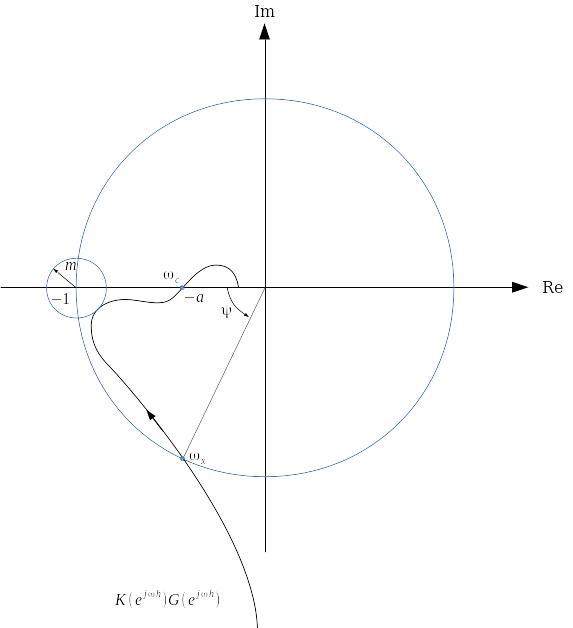
\includegraphics{Images/Chapter7/margins.png}
\caption{Marges de stabilité}
\end{figure}

    Dans la figure ci-dessus, le diagramme de Nyquist présente une
problématique: les marges de gain et de phase indiquent que le système
est très robuste, mais la réalité est que la courbe se rapproche
beaucoup du point critique \(-1\).

Une meilleure mesure de la robustesse pourrait donc être le nombre
\(m\), appelée marge de module.

    \paragraph{Définition (marge de
module)}\label{duxe9finition-marge-de-module}

La marge de module \(m\) est le rayon du plus petit cercle centré au
point critique \(-1\) et tangent à la courbe
\(K(e^{j\omega h})G(e^{j\omega h})\):

\[ m = \inf_{\omega}\left|1 + K(e^{j\omega h})G(e^{j\omega h}) \right| \]

    On accepte souvent une marge de module de \(0.5\)
(\(-6\, \mathrm{dB}\)). On peut aussi montrer aisément (voir figure
suivante) qu'une marge de module \(m\) conduit aux marges de stabilité
suivantes:

\[ M_G > \frac{1}{1-m} \\
   M_P \geq 2\arcsin{\frac{m}{2}}
\]

    \begin{figure}[htbp]
\centering
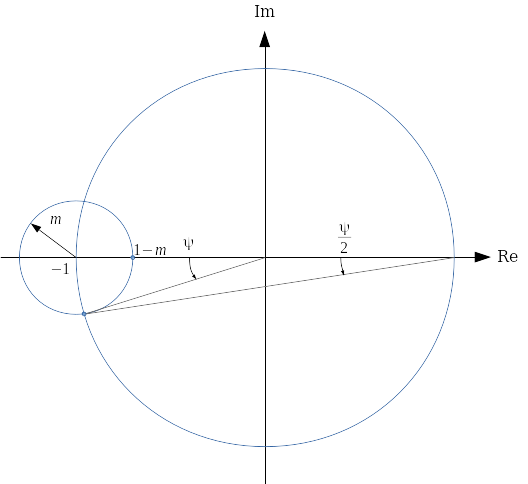
\includegraphics{Images/Chapter7/margins_min.png}
\caption{Marges de stabilité minimum}
\end{figure}

    Il existe un lien direct entre la marge de module et la fonction de
sensibilité:

\[ S(e^{j\omega h}) = \frac{1}{1+K(e^{j\omega h})G(e^{j\omega h})} \]

    D'où:

\[ \left| 1+K(e^{j\omega h})G(e^{j\omega h}) \right| = \frac{1}{\left| S(e^{j\omega h}) \right|} \]

    Et :

\begin{align}
  m &= \inf_{\omega} \left| 1+K(e^{j\omega h})G(e^{j\omega h}) \right| \\
  &= \inf_{\omega} \frac{1}{\left| S(e^{j\omega h}) \right|} \\
  &= \frac{1}{\sup_{\omega} \left| S(e^{j\omega h}) \right|}
\end{align}

    Autrement dit, comme les fonctions harmoniques sont paires et
périodiques de période \(\omega_e\):

\[ \sup_{\omega} \left| S(e^{j\omega h}) \right| = \max_{\omega \in [0,\, \omega_N]} \left| S(e^{j\omega h}) \right| \]

    Et donc:

\[ m = \frac{1}{\max_{\omega \in [0,\, \omega_N]} \left| S(e^{j\omega h}) \right|} \]

    En pratique, il suffit de tracer le diagramme des amplitudes de Bode de
la fonction de sensibilité \(S(e^{j\omega h})\), de mesurer le maximum
de la fonction et d'en prendre l'inverse.

    \paragraph{~Exemple 4}\label{exemple-4}

Soit la fonction de transfert instable en boucle ouverte, avec une
période d'échantillonnage de \(1\, \mathrm{s}\):

\[ K(z)G(z) = K_p \frac{0.015}{z^3(z-0.985} \]

Le calcul des marges peut se faire numériquement.

    \begin{tcolorbox}[breakable, size=fbox, boxrule=1pt, pad at break*=1mm,colback=cellbackground, colframe=cellborder]
\prompt{In}{incolor}{1}{\boxspacing}
\begin{Verbatim}[commandchars=\\\{\}]
\PY{o}{\PYZpc{}}\PY{k}{matplotlib} inline
\PY{k+kn}{import} \PY{n+nn}{matplotlib}\PY{n+nn}{.}\PY{n+nn}{pyplot} \PY{k}{as} \PY{n+nn}{plt}
\PY{n}{plt}\PY{o}{.}\PY{n}{style}\PY{o}{.}\PY{n}{use}\PY{p}{(}\PY{l+s+s1}{\PYZsq{}}\PY{l+s+s1}{../my\PYZus{}params.mplstyle}\PY{l+s+s1}{\PYZsq{}}\PY{p}{)}

\PY{k+kn}{import} \PY{n+nn}{math}
\PY{k+kn}{import} \PY{n+nn}{control}
\end{Verbatim}
\end{tcolorbox}

    \begin{tcolorbox}[breakable, size=fbox, boxrule=1pt, pad at break*=1mm,colback=cellbackground, colframe=cellborder]
\prompt{In}{incolor}{2}{\boxspacing}
\begin{Verbatim}[commandchars=\\\{\}]
\PY{k}{def} \PY{n+nf}{stability\PYZus{}margins}\PY{p}{(}\PY{n}{sys}\PY{p}{,} \PY{n}{omega}\PY{p}{)}\PY{p}{:}
    \PY{k+kn}{import} \PY{n+nn}{scipy}\PY{n+nn}{.}\PY{n+nn}{optimize} \PY{k}{as} \PY{n+nn}{so}
    \PY{k+kn}{import} \PY{n+nn}{numpy} \PY{k}{as} \PY{n+nn}{np}
    
    \PY{n}{wx} \PY{o}{=} \PY{n}{so}\PY{o}{.}\PY{n}{brentq}\PY{p}{(}
        \PY{k}{lambda} \PY{n}{wi}\PY{p}{:} \PY{l+m+mi}{20} \PY{o}{*} \PY{n}{math}\PY{o}{.}\PY{n}{log10}\PY{p}{(}\PY{n}{control}\PY{o}{.}\PY{n}{bode\PYZus{}plot}\PY{p}{(}\PY{n}{H}\PY{p}{,} \PY{p}{[}\PY{n}{wi}\PY{p}{]}\PY{p}{,} \PY{n}{Plot}\PY{o}{=}\PY{k+kc}{False}\PY{p}{)}\PY{p}{[}\PY{l+m+mi}{0}\PY{p}{]}\PY{p}{[}\PY{l+m+mi}{0}\PY{p}{]}\PY{p}{)}\PY{p}{,}
        \PY{n}{omega}\PY{p}{[}\PY{l+m+mi}{0}\PY{p}{]}\PY{p}{,} \PY{n}{omega}\PY{p}{[}\PY{o}{\PYZhy{}}\PY{l+m+mi}{1}\PY{p}{]}
    \PY{p}{)}
    \PY{n}{pm} \PY{o}{=} \PY{l+m+mi}{180} \PY{o}{+} \PY{n}{control}\PY{o}{.}\PY{n}{bode\PYZus{}plot}\PY{p}{(}\PY{n}{H}\PY{p}{,} \PY{n}{Plot}\PY{o}{=}\PY{k+kc}{False}\PY{p}{,} \PY{n}{omega\PYZus{}limits}\PY{o}{=}\PY{p}{[}\PY{n}{omega}\PY{p}{[}\PY{l+m+mi}{0}\PY{p}{]}\PY{p}{,} \PY{n}{wx}\PY{p}{]}\PY{p}{,} \PY{n}{omega\PYZus{}num}\PY{o}{=}\PY{l+m+mi}{10000}\PY{p}{)}\PY{p}{[}\PY{l+m+mi}{1}\PY{p}{]}\PY{p}{[}\PY{o}{\PYZhy{}}\PY{l+m+mi}{1}\PY{p}{]} \PY{o}{*} \PY{l+m+mi}{180} \PY{o}{/} \PY{n}{math}\PY{o}{.}\PY{n}{pi}

    \PY{n}{wc} \PY{o}{=} \PY{n}{so}\PY{o}{.}\PY{n}{brentq}\PY{p}{(}
        \PY{k}{lambda} \PY{n}{wi}\PY{p}{:} \PY{n}{control}\PY{o}{.}\PY{n}{bode\PYZus{}plot}\PY{p}{(}
            \PY{n}{H}\PY{p}{,} \PY{n}{Plot}\PY{o}{=}\PY{k+kc}{False}\PY{p}{,} \PY{n}{omega\PYZus{}limits}\PY{o}{=}\PY{p}{[}\PY{n}{omega}\PY{p}{[}\PY{l+m+mi}{0}\PY{p}{]}\PY{p}{,} \PY{n}{wi}\PY{p}{]}\PY{p}{,} \PY{n}{omega\PYZus{}num}\PY{o}{=}\PY{l+m+mi}{10000}
        \PY{p}{)}\PY{p}{[}\PY{l+m+mi}{1}\PY{p}{]}\PY{p}{[}\PY{o}{\PYZhy{}}\PY{l+m+mi}{1}\PY{p}{]} \PY{o}{+} \PY{n}{math}\PY{o}{.}\PY{n}{pi}\PY{p}{,}
        \PY{n}{omega}\PY{p}{[}\PY{l+m+mi}{0}\PY{p}{]}\PY{p}{,} \PY{n}{omega}\PY{p}{[}\PY{o}{\PYZhy{}}\PY{l+m+mi}{1}\PY{p}{]}
    \PY{p}{)}
    \PY{n}{gm} \PY{o}{=} \PY{o}{\PYZhy{}}\PY{l+m+mi}{20} \PY{o}{*} \PY{n}{math}\PY{o}{.}\PY{n}{log10}\PY{p}{(}\PY{n}{control}\PY{o}{.}\PY{n}{bode\PYZus{}plot}\PY{p}{(}\PY{n}{H}\PY{p}{,} \PY{p}{[}\PY{n}{wc}\PY{p}{]}\PY{p}{,} \PY{n}{Plot}\PY{o}{=}\PY{k+kc}{False}\PY{p}{)}\PY{p}{[}\PY{l+m+mi}{0}\PY{p}{]}\PY{p}{[}\PY{l+m+mi}{0}\PY{p}{]}\PY{p}{)}
    
    \PY{n}{D} \PY{o}{=} \PY{l+m+mi}{1} \PY{o}{+} \PY{n}{sys}
    \PY{n}{mag}\PY{p}{,} \PY{n}{phase}\PY{p}{,} \PY{n}{omega} \PY{o}{=} \PY{n}{control}\PY{o}{.}\PY{n}{bode\PYZus{}plot}\PY{p}{(}\PY{n}{D}\PY{p}{,} \PY{n}{Plot}\PY{o}{=}\PY{k+kc}{False}\PY{p}{,} \PY{n}{omega\PYZus{}limits}\PY{o}{=}\PY{p}{[}\PY{n}{omega}\PY{p}{[}\PY{l+m+mi}{0}\PY{p}{]}\PY{p}{,} \PY{n}{omega}\PY{p}{[}\PY{o}{\PYZhy{}}\PY{l+m+mi}{1}\PY{p}{]}\PY{p}{]}\PY{p}{,} \PY{n}{omega\PYZus{}num}\PY{o}{=}\PY{l+m+mi}{100000}\PY{p}{)}
    
    \PY{n}{i} \PY{o}{=} \PY{n}{np}\PY{o}{.}\PY{n}{argmin}\PY{p}{(}\PY{n}{mag}\PY{p}{)}
    \PY{n}{sm}\PY{p}{,} \PY{n}{ws} \PY{o}{=} \PY{l+m+mi}{20} \PY{o}{*} \PY{n}{math}\PY{o}{.}\PY{n}{log10}\PY{p}{(}\PY{n}{mag}\PY{p}{[}\PY{n}{i}\PY{p}{]}\PY{p}{)}\PY{p}{,} \PY{n}{omega}\PY{p}{[}\PY{n}{i}\PY{p}{]}
    
    \PY{k}{return} \PY{n}{gm}\PY{p}{,} \PY{n}{pm}\PY{p}{,} \PY{n}{sm}\PY{p}{,} \PY{n}{wc}\PY{p}{,} \PY{n}{wx}\PY{p}{,} \PY{n}{ws}
\end{Verbatim}
\end{tcolorbox}

    \begin{tcolorbox}[breakable, size=fbox, boxrule=1pt, pad at break*=1mm,colback=cellbackground, colframe=cellborder]
\prompt{In}{incolor}{3}{\boxspacing}
\begin{Verbatim}[commandchars=\\\{\}]
\PY{n}{Kp} \PY{o}{=} \PY{l+m+mi}{25}  \PY{c+c1}{\PYZsh{} try 6.7 and 25}
\PY{n}{H} \PY{o}{=} \PY{n}{control}\PY{o}{.}\PY{n}{tf}\PY{p}{(}\PY{p}{[}\PY{n}{Kp} \PY{o}{*} \PY{l+m+mf}{0.015}\PY{p}{]}\PY{p}{,} \PY{p}{[}\PY{l+m+mi}{1}\PY{p}{,} \PY{o}{\PYZhy{}}\PY{l+m+mf}{0.985}\PY{p}{,} \PY{l+m+mi}{0}\PY{p}{,} \PY{l+m+mi}{0}\PY{p}{,} \PY{l+m+mi}{0}\PY{p}{]}\PY{p}{,} \PY{l+m+mi}{1}\PY{p}{)}

\PY{n}{mag}\PY{p}{,} \PY{n}{phase}\PY{p}{,} \PY{n}{omega} \PY{o}{=} \PY{n}{control}\PY{o}{.}\PY{n}{bode\PYZus{}plot}\PY{p}{(}\PY{n}{H}\PY{p}{,} \PY{n}{dB}\PY{o}{=}\PY{k+kc}{True}\PY{p}{,} \PY{n}{omega\PYZus{}limits}\PY{o}{=}\PY{p}{[}\PY{l+m+mf}{1e\PYZhy{}3}\PY{p}{,} \PY{n}{math}\PY{o}{.}\PY{n}{pi}\PY{p}{]}\PY{p}{,} \PY{n}{omega\PYZus{}num}\PY{o}{=}\PY{l+m+mi}{100000}\PY{p}{)}

\PY{n}{mag} \PY{o}{=} \PY{p}{[}\PY{l+m+mi}{20} \PY{o}{*} \PY{n}{math}\PY{o}{.}\PY{n}{log10}\PY{p}{(}\PY{n}{m}\PY{p}{)} \PY{k}{for} \PY{n}{m} \PY{o+ow}{in} \PY{n}{mag}\PY{p}{]}
\PY{n}{phase} \PY{o}{=} \PY{p}{[}\PY{n}{p} \PY{o}{*} \PY{l+m+mi}{180} \PY{o}{/} \PY{n}{math}\PY{o}{.}\PY{n}{pi} \PY{k}{for} \PY{n}{p} \PY{o+ow}{in} \PY{n}{phase}\PY{p}{]}
\end{Verbatim}
\end{tcolorbox}

    \begin{center}
    \adjustimage{max size={0.9\linewidth}{0.9\paperheight}}{Chapter7_Stability_files/Chapter7_Stability_63_0.png}
    \end{center}
    { \hspace*{\fill} \\}
    
    \begin{tcolorbox}[breakable, size=fbox, boxrule=1pt, pad at break*=1mm,colback=cellbackground, colframe=cellborder]
\prompt{In}{incolor}{4}{\boxspacing}
\begin{Verbatim}[commandchars=\\\{\}]
\PY{n}{gm}\PY{p}{,} \PY{n}{pm}\PY{p}{,} \PY{n}{sm}\PY{p}{,} \PY{n}{wc}\PY{p}{,} \PY{n}{wx}\PY{p}{,} \PY{n}{ws} \PY{o}{=} \PY{n}{stability\PYZus{}margins}\PY{p}{(}\PY{n}{H}\PY{p}{,} \PY{n}{omega}\PY{p}{)}

\PY{n+nb}{print}\PY{p}{(}\PY{l+s+s1}{\PYZsq{}}\PY{l+s+s1}{Marge de gain: }\PY{l+s+si}{\PYZob{}:.2f\PYZcb{}}\PY{l+s+s1}{ dB à }\PY{l+s+si}{\PYZob{}:.2f\PYZcb{}}\PY{l+s+s1}{ rad/s}\PY{l+s+s1}{\PYZsq{}}\PY{o}{.}\PY{n}{format}\PY{p}{(}\PY{n}{gm}\PY{p}{,} \PY{n}{wc}\PY{p}{)}\PY{p}{)}
\PY{n+nb}{print}\PY{p}{(}\PY{l+s+s1}{\PYZsq{}}\PY{l+s+s1}{Marge de phase: }\PY{l+s+si}{\PYZob{}:.2f\PYZcb{}}\PY{l+s+s1}{ deg à }\PY{l+s+si}{\PYZob{}:.2f\PYZcb{}}\PY{l+s+s1}{ rad/s}\PY{l+s+s1}{\PYZsq{}}\PY{o}{.}\PY{n}{format}\PY{p}{(}\PY{n}{pm}\PY{p}{,} \PY{n}{wx}\PY{p}{)}\PY{p}{)}
\PY{n+nb}{print}\PY{p}{(}\PY{l+s+s1}{\PYZsq{}}\PY{l+s+s1}{Marge de retard: }\PY{l+s+si}{\PYZob{}:.2f\PYZcb{}}\PY{l+s+s1}{ s}\PY{l+s+s1}{\PYZsq{}}\PY{o}{.}\PY{n}{format}\PY{p}{(}\PY{n}{pm}\PY{o}{/}\PY{n}{wx}\PY{o}{*}\PY{n}{math}\PY{o}{.}\PY{n}{pi}\PY{o}{/}\PY{l+m+mi}{180}\PY{p}{)}\PY{p}{)}
\PY{n+nb}{print}\PY{p}{(}\PY{l+s+s1}{\PYZsq{}}\PY{l+s+s1}{Marge de module: }\PY{l+s+si}{\PYZob{}:.2f\PYZcb{}}\PY{l+s+s1}{ dB}\PY{l+s+s1}{\PYZsq{}}\PY{o}{.}\PY{n}{format}\PY{p}{(}\PY{n}{sm}\PY{p}{)}\PY{p}{)}
\end{Verbatim}
\end{tcolorbox}

    \begin{Verbatim}[commandchars=\\\{\}]
Marge de gain: 1.60 dB à 0.46 rad/s
Marge de phase: 16.08 deg à 0.38 rad/s
Marge de retard: 0.74 s
Marge de module: -16.66 dB
    \end{Verbatim}

    Si le retard réel était de \(4\, \mathrm{s}\) au lieu de \(3\), le
système pour \(K_p = 25\) deviendrait instable car la marge de retard
est inférieure à l'erreur!

    \subsection{7.6 Ecarts permanents}\label{ecarts-permanents}

    \subsubsection{Montage en
asservissement}\label{montage-en-asservissement}

    Après l'atténuation du régime transitoire, il peut subsister ou non un
écart entre la consigne et la sortie du processus. Cet écart est appelé
écart permanent d'asservissement et est défini comme la limite, pour
\(k\) tendant vers l'infini, de l'écart \(e(k) = y_c(k) - y(k)\).

La fonction de transfert reliant l'erreur à la consigne est rappelée
ici:

\begin{align}
  E(z) &= \frac{1}{1+K(z)G(z)} Y_c(z) \\
       &= S(z) Y_c(z)
\end{align}

Le système étant supposé stable à ce stade de l'étude, les zéros de
\(1+K(z)G(z)\) sont tous à l'intérieur du cercle unité.

    La fonction de transfert en boucle ouverte est réécrite en faisant
apparaître le pôle \(z=1\) de multiplicité \(l\) (soit l intégrateurs):

\[ K(z)G(z) = \frac{B(z)}{(z-1)^l A(z)} \]

    \paragraph{Définition}\label{duxe9finition}

L'entier \(l\) est appelé type ou classe du système en boucle ouverte.
***

    \paragraph{Définition}\label{duxe9finition}

Le gain permanent du système en boucle ouverte est le nombre:

\[ \gamma = \lim_{z \rightarrow 1} (z-1)^l K(z)G(z) = \frac{B(1)}{A(1)} \]
***

    Lorsque \(l = 0\), \(l = 1\) et \(l = 2\), \(\gamma\) porte
respectivement les dénominations gain statique, en vitesse et en
accélération.

    \paragraph{Exemple}\label{exemple}

Pour \(l=0\), lorsque la consigne est un saut unité discret, on obtient:

\begin{align}
  E(z) &= \frac{1}{1+K(z)G(z)} \frac{z}{z-1} \\
       &= \frac{1}{1 + \frac{B(z)}{A(z)}} \frac{z}{z-1}
\end{align}

Et donc, par le théorème de la valeur finale:

\[ \lim_{k \rightarrow \infty} e(k) = \lim_{z \rightarrow 1} (z-1) \frac{1}{1+K(z)G(z)} \frac{z}{z-1} = \frac{1}{1+\gamma} \]
***

    Ce type de tableau ayant déjà été construit dans le cours d'analyse des
systèmes continus, seul le tableau final est donné. L'étudiant est
invité à le démontrer lui-même comme exercice.

    \begin{longtable}[]{@{}cccc@{}}
\toprule
\begin{minipage}[b]{0.3\columnwidth}\centering\strut
\[ \frac{\text{Consigne}}{\text{Type du système en BO}} \]\strut
\end{minipage} & \begin{minipage}[b]{0.15\columnwidth}\centering\strut
\[ y_c(k) = 1 \]\strut
\end{minipage} & \begin{minipage}[b]{0.15\columnwidth}\centering\strut
\[ y_c(k) = kh \]\strut
\end{minipage} & \begin{minipage}[b]{0.15\columnwidth}\centering\strut
\[ y_c(k) = \frac{1}{2}(kh)^2 \]\strut
\end{minipage}\tabularnewline
\midrule
\endhead
\begin{minipage}[t]{0.3\columnwidth}\centering\strut
\[ 0 \]\strut
\end{minipage} & \begin{minipage}[t]{0.15\columnwidth}\centering\strut
\[ \text{Statisme}\, \frac{1}{1+\gamma} \]\strut
\end{minipage} & \begin{minipage}[t]{0.15\columnwidth}\centering\strut
\[ \infty \]\strut
\end{minipage} & \begin{minipage}[t]{0.15\columnwidth}\centering\strut
\[ \infty \]\strut
\end{minipage}\tabularnewline
\begin{minipage}[t]{0.3\columnwidth}\centering\strut
\[ 1 \]\strut
\end{minipage} & \begin{minipage}[t]{0.15\columnwidth}\centering\strut
\[ 0 \]\strut
\end{minipage} & \begin{minipage}[t]{0.15\columnwidth}\centering\strut
\[ \text{Traînée}\, \frac{h}{\gamma} \]\strut
\end{minipage} & \begin{minipage}[t]{0.15\columnwidth}\centering\strut
\[ \infty \]\strut
\end{minipage}\tabularnewline
\begin{minipage}[t]{0.3\columnwidth}\centering\strut
\[ 2 \]\strut
\end{minipage} & \begin{minipage}[t]{0.15\columnwidth}\centering\strut
\[ 0 \]\strut
\end{minipage} & \begin{minipage}[t]{0.15\columnwidth}\centering\strut
\[ 0 \]\strut
\end{minipage} & \begin{minipage}[t]{0.15\columnwidth}\centering\strut
\[ \frac{h^2}{\gamma} \]\strut
\end{minipage}\tabularnewline
\bottomrule
\end{longtable}

    On remarque aisément qu'au plus \(\gamma\) est grand, au plus l'écart
permanent d'asservissement sera faible. Cependant, un grand gain
permanent signifie aussi des marges de stabilité plus faibles. On voit
donc apparaître clairement un dilemme précision-stabilité.

    \subsubsection{Montage en régulation}\label{montage-en-ruxe9gulation}

    Suite à une perturbation, le système dynamique passe par une phase
transitoire et fini par se stabiliser (on suppose à nouveau le système
BIBO stable). Il peut, comme dans le cas précédent, subsister ou non un
écart permanent de régulation, défini comme
\(\lim_{k \rightarrow \infty} -y(k)\).

    Dans ce cas, les pôles \(z=1\) sont mis en évidence pour le système
ainsi que le régulateur.

    \[ K(z) = \frac{S(z)}{(z-1)^l R(z)} \]

\[ G(z) = \frac{B(z)}{(z-1)^{l'} A(z)} \]

    \paragraph{Définition}\label{duxe9finition}

L'entier \(l'\) est appelé type ou classe du régulateur. ***

    \paragraph{Définition}\label{duxe9finition}

Le gain permanent du régulateur est le nombre:

\[ \gamma = \lim_{z \rightarrow 1} (z-1)^l K(z) = \frac{S(1)}{R(1)} \]
***

    Dans les définitions précédentes, le régulateur désigne seulement
l'élément positionné en amont de la perturbation.

    Pour les mêmes raisons que le tableau des erreurs d'asservissement, le
tableau final est donné sans développement. L'étudiant est invité à le
démontrer comme exercice. Attention tout de même au fait que la
perturbation étant d'origine analogique, elle ne peut être discrétisée
qu'à condition d'être lente ou constante.

    \begin{longtable}[]{@{}cccc@{}}
\toprule
\begin{minipage}[b]{0.2\columnwidth}\centering\strut
\[ \frac{\text{Perturbation}}{\text{Type du régulateur}} \]\strut
\end{minipage} & \begin{minipage}[b]{0.35\columnwidth}\centering\strut
\[ w(k) = 1 \]\strut
\end{minipage} & \begin{minipage}[b]{0.15\columnwidth}\centering\strut
\[ w(k) = kh \]\strut
\end{minipage} & \begin{minipage}[b]{0.15\columnwidth}\centering\strut
\[ w(k) = \frac{1}{2}(kh)^2 \]\strut
\end{minipage}\tabularnewline
\midrule
\endhead
\begin{minipage}[t]{0.2\columnwidth}\centering\strut
\[ 0 \]\strut
\end{minipage} & \begin{minipage}[t]{0.35\columnwidth}\centering\strut
\[ \text{Statisme}\, \left\{ \begin{array}{rl} -\frac{G(1)}{1+K(1)G(1)} \quad \text{si}\: l' = 0 \\ -\frac{1}{K(1)} \quad \text{si}\: l' > 0 \end{array} \right. \]\strut
\end{minipage} & \begin{minipage}[t]{0.15\columnwidth}\centering\strut
\[ \infty \]\strut
\end{minipage} & \begin{minipage}[t]{0.15\columnwidth}\centering\strut
\[ \infty \]\strut
\end{minipage}\tabularnewline
\begin{minipage}[t]{0.2\columnwidth}\centering\strut
\[ 1 \]\strut
\end{minipage} & \begin{minipage}[t]{0.35\columnwidth}\centering\strut
\[ 0 \]\strut
\end{minipage} & \begin{minipage}[t]{0.15\columnwidth}\centering\strut
\[ -\frac{h}{\gamma} \]\strut
\end{minipage} & \begin{minipage}[t]{0.15\columnwidth}\centering\strut
\[ \infty \]\strut
\end{minipage}\tabularnewline
\begin{minipage}[t]{0.2\columnwidth}\centering\strut
\[ 2 \]\strut
\end{minipage} & \begin{minipage}[t]{0.35\columnwidth}\centering\strut
\[ 0 \]\strut
\end{minipage} & \begin{minipage}[t]{0.15\columnwidth}\centering\strut
\[ 0 \]\strut
\end{minipage} & \begin{minipage}[t]{0.15\columnwidth}\centering\strut
\[ -\frac{h^2}{\gamma} \]\strut
\end{minipage}\tabularnewline
\bottomrule
\end{longtable}

    On remarque à nouveau qu'au plus les gains sont élevés, au plus la
précision sera meilleure.

    Il est à remarquer que les montages en asservissement et en régulation
ne se comportent pas exactement de la même manière. Alors que les écarts
permanents d'asservissement dépendent de l'entièreté de la boucle
ouverte, les écarts permanent de régulation, eux, dépendent
principalement du régulateur positionné en amont de la perturbation.

    \paragraph{Exemple}\label{exemple}

Soit un moteur DC, commandé en position, dont la fonction de transfert
est:

\[ G(s) = \frac{4}{s(s+2)} \]

Ce moteur est commandé par un régulateur proportionnel de gain \(K_p\).

    On a donc, après échantillonnage de la fonction de transfert du moteur
pour \(h = 0.025\, \mathrm{s}\):

\[ K(z) = K_p \]

\[ G(z) = \frac{10^{-3}(1.23z+1.21)}{(z-1)(z-0.95)} \]

Le régulateur est de type 0 et le moteur de type 1.

    D'après les tableaux, comme le type de la boucle ouverte est de 1, le
statisme d'asservissement est nul pour une consigne en forme d'échelon,
alors que le statisme de régulation vaut \(-1/K_p\) pour une
perturbation constante.

    \subsection{7.7 Principe des vases
communicants}\label{principe-des-vases-communicants}

    \paragraph{~Théorème}\label{thuxe9oruxe8me}

Soient un système stable en boucle fermée et
\(p_i, \, i=1, 2, \dots, P\), les pôles de \(K(z)G(z)\) à l'extérieur du
cercle unité, en comptant leurs multiplicités. La fonction de transfert
\(K(z)G(z)\) est supposée strictement propre. Alors la fonction de
sensibilité harmonique satisfait l'égalité:

\[ \int_0^{\omega_N} \log \left| S(e^{j\omega h})\right| d\omega = \omega_N \sum_{i=1}^{P} \log |p_i| \]

    En français, cela signifie que la surface sous la courbe des gains de la
fonction de sensibilité \(S(z)\) est égale à une constante inhérente au
système en boucle ouverte, valant la somme des amplitudes des pôles
instables de ce dernier mutlipliés par \(\omega_N\).

Autrement dit, quoique nous fassions, la fonction de sensibilité
possédera une allure telle que, dans l'intervalle \([0, \omega_N]\), la
surface sera constante. Cela aura pour conséquence que si on crée une
grande surface négative d'un côté de l'interval, une surface positive
proportionnelle sera générée de l'autre côté. Cela se fera évidemment
par l'apparition d'un pic de sensibilité.

Attention tout de même que l'égalité est définie pour un graphique dont
le gain est défini en décibels, et les 2 axes étant linéaires.

    Voyons maintenant en quoi ce principe des vases communicants est
important.

    Rappelons tout d'abord que la robustesse dépend de la marge de module:

\[ m = \frac{1}{\max_{\omega \in [0, \omega_N]} \left| S(e^{j\omega h})\right|} \]

Il faut donc, pour avoir une bonne marge de module, et donc une bonne
robustesse, que le pic de sensibilité soit le plus faible possible.

    Cependant, pour avoir une bonne précision en régime permanent en boucle
fermée, il faut augmenter les gains afin que la fonction de sensibilité
soit proche de 0, car:

\[ \frac{E(z)}{Y_c(z)} = \frac{1}{1+K(z)G(z)} = S(z) \]

    Le régime permanent étant souvent en basse fréquence, cela signifie que
le terme \(\left| 1 + K(z)G(z) \right|\) doit être le plus élevé
possible à basse fréquence. Cela crée donc une surface négative
importante dans le diagramme de \(\left| S(e^{j\omega h}) \right|\), du
côté des basses fréquences. Comme, en général, on aimerait que la bande
passante soit la plus grande possible, on essaye de garder des grands
gains sur une large plage de fréquences. Mais alors, par le théorème
plus haut, afin que l'égalité soit respectée, il faut générer une
surface positive importante du côté des hautes fréquences. Au plus la
plage de fréquence en dehors de la bande passante imposée sera faible,
au plus, afin de garantir l'égalité, le pic de sensibilité sera élevé.
Cela a pour impact une très mauvaise marge de module.

    Ce théorème permet de comprendre pourquoi un système instable est
difficile à contrôler avec des marges suffisantes. En effet, le second
membre de l'égalité devient positif, imposant à la courbe de sensibilité
d'avoir une surface positive plus importante que la surface négative.

    \paragraph{Exemple}\label{exemple}

Soit le système suivant, avec \(h=1\, \mathrm{s}\):

\[ K(z)G(z) = K_p \frac{0.015}{z^3(z-0.985)} \]

    Comme le système ne possède aucun pôle instable, le théorème donne:

\[ \int_0^{\pi} \log \left| S(e^{j\omega h})\right| d\omega = 0 \]

    \begin{tcolorbox}[breakable, size=fbox, boxrule=1pt, pad at break*=1mm,colback=cellbackground, colframe=cellborder]
\prompt{In}{incolor}{5}{\boxspacing}
\begin{Verbatim}[commandchars=\\\{\}]
\PY{n}{Kp} \PY{o}{=} \PY{p}{[}\PY{l+m+mf}{6.7}\PY{p}{,} \PY{l+m+mi}{25}\PY{p}{]}

\PY{n}{fig}\PY{p}{,} \PY{n}{ax} \PY{o}{=} \PY{n}{plt}\PY{o}{.}\PY{n}{subplots}\PY{p}{(}\PY{p}{)}

\PY{k}{for} \PY{n}{k} \PY{o+ow}{in} \PY{n}{Kp}\PY{p}{:}
    \PY{n}{H} \PY{o}{=} \PY{n}{control}\PY{o}{.}\PY{n}{tf}\PY{p}{(}\PY{p}{[}\PY{n}{k} \PY{o}{*} \PY{l+m+mf}{0.015}\PY{p}{]}\PY{p}{,} \PY{p}{[}\PY{l+m+mi}{1}\PY{p}{,} \PY{o}{\PYZhy{}}\PY{l+m+mf}{0.985}\PY{p}{,} \PY{l+m+mi}{0}\PY{p}{,} \PY{l+m+mi}{0}\PY{p}{,} \PY{l+m+mi}{0}\PY{p}{]}\PY{p}{,} \PY{l+m+mi}{1}\PY{p}{)}

    \PY{n}{S} \PY{o}{=} \PY{l+m+mi}{1} \PY{o}{/} \PY{p}{(}\PY{l+m+mi}{1} \PY{o}{+} \PY{n}{H}\PY{p}{)}
    \PY{n}{mag}\PY{p}{,} \PY{n}{phase}\PY{p}{,} \PY{n}{omega} \PY{o}{=} \PY{n}{control}\PY{o}{.}\PY{n}{bode\PYZus{}plot}\PY{p}{(}\PY{n}{S}\PY{p}{,} \PY{n}{Plot}\PY{o}{=}\PY{k+kc}{False}\PY{p}{,} \PY{n}{omega\PYZus{}limits}\PY{o}{=}\PY{p}{[}\PY{l+m+mf}{1e\PYZhy{}3}\PY{p}{,} \PY{n}{math}\PY{o}{.}\PY{n}{pi}\PY{p}{]}\PY{p}{,} \PY{n}{omega\PYZus{}num}\PY{o}{=}\PY{l+m+mi}{100000}\PY{p}{)}

    \PY{n}{mag} \PY{o}{=} \PY{p}{[}\PY{l+m+mi}{20} \PY{o}{*} \PY{n}{math}\PY{o}{.}\PY{n}{log10}\PY{p}{(}\PY{n}{m}\PY{p}{)} \PY{k}{for} \PY{n}{m} \PY{o+ow}{in} \PY{n}{mag}\PY{p}{]}

    \PY{n}{ax}\PY{o}{.}\PY{n}{plot}\PY{p}{(}\PY{n}{omega}\PY{p}{,} \PY{n}{mag}\PY{p}{,} \PY{n}{label}\PY{o}{=}\PY{l+s+s1}{\PYZsq{}}\PY{l+s+s1}{Kp=}\PY{l+s+si}{\PYZob{}\PYZcb{}}\PY{l+s+s1}{\PYZsq{}}\PY{o}{.}\PY{n}{format}\PY{p}{(}\PY{n}{k}\PY{p}{)}\PY{p}{)}

    \PY{n+nb}{print}\PY{p}{(}\PY{l+s+s1}{\PYZsq{}}\PY{l+s+s1}{La marge de module pour Kp = }\PY{l+s+si}{\PYZob{}\PYZcb{}}\PY{l+s+s1}{ vaut: }\PY{l+s+si}{\PYZob{}\PYZcb{}}\PY{l+s+s1}{\PYZsq{}}\PY{o}{.}\PY{n}{format}\PY{p}{(}\PY{n}{k}\PY{p}{,} \PY{o}{\PYZhy{}}\PY{n+nb}{max}\PY{p}{(}\PY{n}{mag}\PY{p}{)}\PY{p}{)}\PY{p}{)}

\PY{n}{\PYZus{}} \PY{o}{=} \PY{n}{ax}\PY{o}{.}\PY{n}{legend}\PY{p}{(}\PY{p}{)}
\end{Verbatim}
\end{tcolorbox}

    \begin{Verbatim}[commandchars=\\\{\}]
La marge de module pour Kp = 6.7 vaut: -2.653020122061182
La marge de module pour Kp = 25 vaut: -16.662833773879168
    \end{Verbatim}

    \begin{center}
    \adjustimage{max size={0.9\linewidth}{0.9\paperheight}}{Chapter7_Stability_files/Chapter7_Stability_101_1.png}
    \end{center}
    { \hspace*{\fill} \\}
    
    On remarque qu'en augmentant le gain \(K_p\), le minimum de
\(S(e^{j\omega h})\), obtenu pour \(\omega = 0\), est beaucoup plus
faible. Cela se traduit donc par une très faible sensibilité de l'erreur
par rapport à l'entrée. L'erreur est donc proche de 0 pour une entrée
basse fréquence.

Le pic de sensibilité aussi augmente considérablement avec \(K_p\),
engendrant une piètre marge de robustesse.



    % Add a bibliography block to the postdoc
    
    
    
\end{document}
